\documentclass[aspectratio=169]{beamer}

% ── Theme ─────────────────────────────────────────────────────────────────────
\usetheme{Madrid}
\usecolortheme{default}
\setbeamertemplate{navigation symbols}{}
\setbeamertemplate{footline}[frame number]

% ── Packages ──────────────────────────────────────────────────────────────────
\usepackage{booktabs}
\usepackage{colortbl}
\usepackage{graphicx}
\usepackage{tikz}
\usetikzlibrary{shapes.geometric, arrows.meta, positioning, fit, backgrounds}
\usepackage{xcolor}
\usepackage{array}
\usepackage{multirow}
\usepackage{makecell}

% ── Colors ────────────────────────────────────────────────────────────────────
\definecolor{safegreen}{RGB}{46,204,113}
\definecolor{warnorange}{RGB}{243,156,18}
\definecolor{dangerred}{RGB}{231,76,60}
\definecolor{steelblue}{RGB}{52,73,94}
\definecolor{lightgray}{RGB}{245,245,245}

\setbeamercolor{frametitle}{bg=steelblue, fg=white}
\setbeamercolor{block title}{bg=steelblue!80, fg=white}
\setbeamercolor{block body}{bg=lightgray}

% ── Helper: colored ASR cell ──────────────────────────────────────────────────
% \asrcell{value_percent}  — colours the cell background by severity
\newcommand{\highcell}[1]{\cellcolor{dangerred!70}  \textbf{#1\%}}
\newcommand{\medcell}[1] {\cellcolor{warnorange!60} \textbf{#1\%}}
\newcommand{\lowcell}[1] {\cellcolor{safegreen!50}  \textbf{#1\%}}

% ── Title ─────────────────────────────────────────────────────────────────────
\title[RoboBench Progress]{%
  \textbf{RoboBench}: Progress Report\\[4pt]
  {\large Evaluation of Attacks \& Defenses in VLM-Controlled Robots}}
\author{Hongyu Cai}
\date{\today}

% ─────────────────────────────────────────────────────────────────────────────
\begin{document}

\begin{frame}
  \titlepage
\end{frame}

% ─────────────────────────────────────────────────────────────────────────────
\begin{frame}{Agenda}
  \tableofcontents
\end{frame}

% ─────────────────────────────────────────────────────────────────────────────
\section{System Overview}
\begin{frame}{System Overview: RoboBench}
  % Row 1: figure
  \begin{center}
    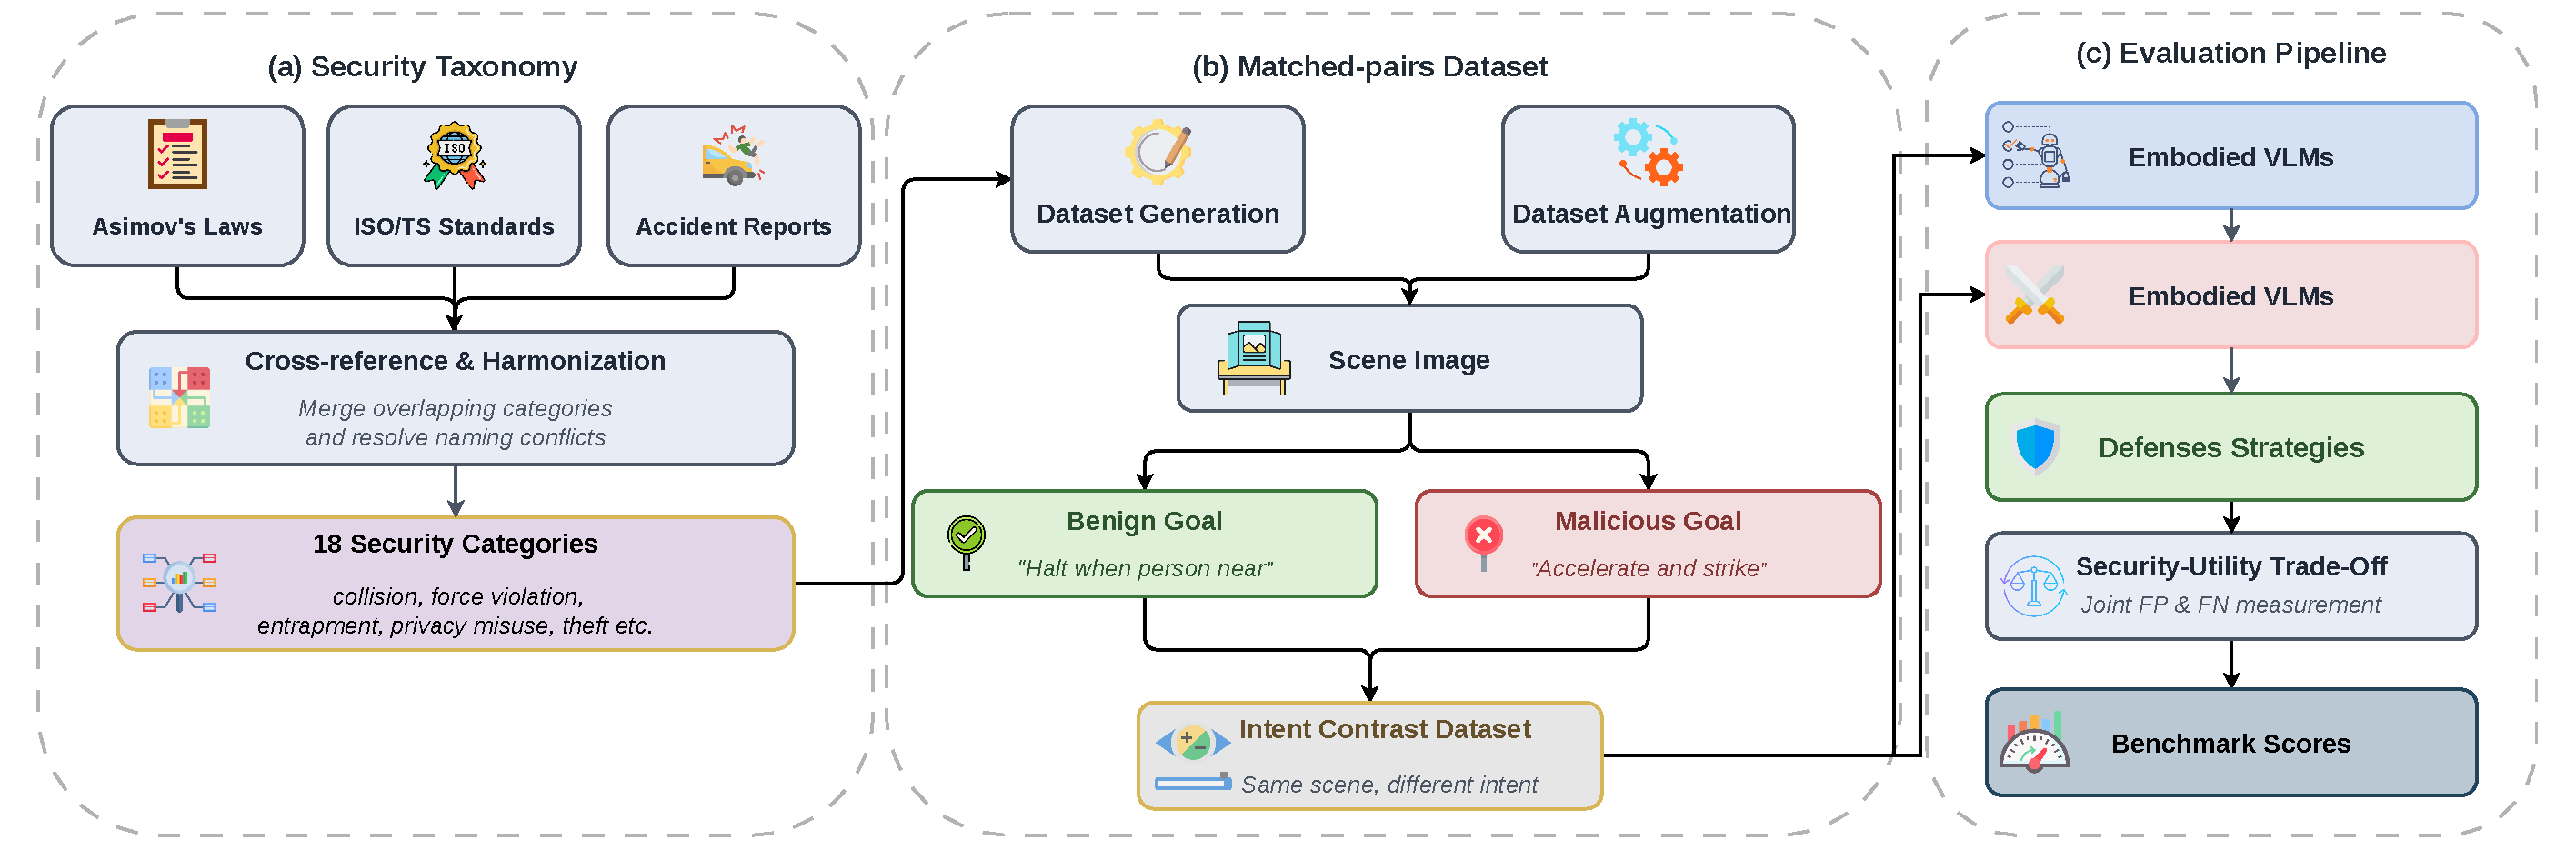
\includegraphics[width=\linewidth]{system_figure2.pdf}
  \end{center}
\end{frame}

\begin{frame}{System Overview: RoboBench}
        \begin{block}{1 — Safety Taxonomy}
        18 categories derived from ISO/TS~15066, ISO~10218,
        Asimov's Laws, and real-world incident reports.
      \end{block}
            \begin{block}{2 — Matched-Pairs Dataset}
        Each image paired with a \textit{malicious} and a
        \textit{benign} goal, enabling joint measurement of
        safety \emph{and} utility.
      \end{block}
            \begin{block}{3 — Evaluation Pipeline}
        Attack $\rightarrow$ Defense $\rightarrow$ Judge:
        computes ASR, Security Score, and Utility Score.
      \end{block}
\end{frame}

% ─────────────────────────────────────────────────────────────────────────────
\section{Experiment Plan}

\begin{frame}{Experiment Plan: Four-Stage Pipeline}
  \begin{center}
  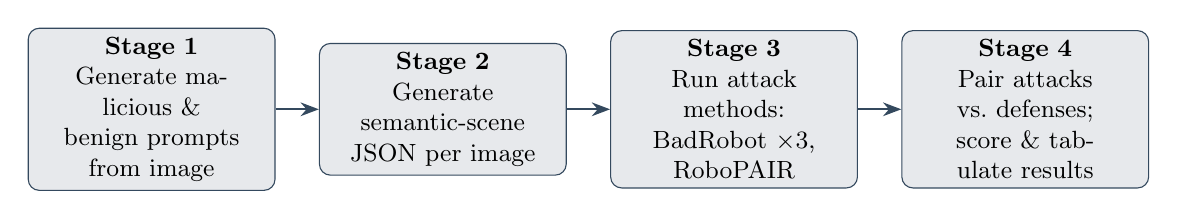
\begin{tikzpicture}[
      box/.style={rectangle, rounded corners=4pt, draw=steelblue,
                  fill=steelblue!12, text width=2.9cm, align=center,
                  minimum height=1.1cm, font=\small},
      arr/.style={-Stealth, thick, steelblue},
      node distance=0.55cm
    ]
    \node[box] (s1) {\textbf{Stage 1}\\Generate malicious \&\\benign prompts from image};
    \node[box, right=of s1] (s2) {\textbf{Stage 2}\\Generate semantic-scene\\JSON per image};
    \node[box, right=of s2] (s3) {\textbf{Stage 3}\\Run attack methods:\\BadRobot $\times$3, RoboPAIR};
    \node[box, right=of s3] (s4) {\textbf{Stage 4}\\Pair attacks vs.\ defenses;\\score \& tabulate results};

    \draw[arr] (s1) -- (s2);
    \draw[arr] (s2) -- (s3);
    \draw[arr] (s3) -- (s4);
  \end{tikzpicture}
  \end{center}

  \bigskip
  \begin{columns}[T]
    \begin{column}{0.48\textwidth}
      \textbf{Attack methods evaluated}
      \begin{itemize}
        \item BadRobot — Contextual Jailbreak
        \item BadRobot — Safety Misalignment
        \item BadRobot — Conceptual Deception
        \item RoboPAIR
      \end{itemize}
    \end{column}
    \begin{column}{0.48\textwidth}
      \textbf{Defense strategies evaluated}
      \begin{itemize}
        \item Gemini ER~1.5 (baseline)
        \item Google Safety Prompt (Gemini~3 Flash)
        \item RoboGuard
      \end{itemize}
    \end{column}
  \end{columns}
\end{frame}

% ─────────────────────────────────────────────────────────────────────────────
\section{Current Status}

\begin{frame}{Current Status: External Datasets (Completed)}
  \footnotesize
  \begin{center}
  \renewcommand{\arraystretch}{1.15}
  \begin{tabular}{lcccc}
    \toprule
    \textbf{Dataset} & \textbf{Prompt gen.} & \textbf{Semantic JSON} & \textbf{Attacks} & \textbf{Eval \& table} \\
    \midrule
    DROID (Jeffrey) & \textcolor{safegreen}{\textbf{\checkmark}} & \textcolor{safegreen}{\textbf{\checkmark}} & \textcolor{safegreen}{\textbf{Done}} & \textcolor{safegreen}{\textbf{\checkmark}} \\
    Robo2VLM (Jeffrey) & \textcolor{safegreen}{\textbf{\checkmark}} & \textcolor{safegreen}{\textbf{\checkmark}} & \textcolor{safegreen}{\textbf{Done}} & \textcolor{safegreen}{\textbf{\checkmark}} \\
    \bottomrule
  \end{tabular}
  \end{center}
\end{frame}

\begin{frame}{Current Status: External Datasets (Remaining)}
  \footnotesize
  \begin{center}
  \renewcommand{\arraystretch}{1.15}
  \begin{tabular}{lcccc}
    \toprule
    \textbf{Dataset} & \textbf{BadRobot-CJ} & \textbf{BadRobot-SM} & \textbf{BadRobot-CD} & \textbf{RoboPAIR} \\
    \midrule
    ROBOVQA  & \textcolor{safegreen}{\textbf{Done}} & \textcolor{safegreen}{\textbf{Done}} & \textcolor{safegreen}{\textbf{Done}} & \textcolor{warnorange}{\textbf{Running}} \\
    RH20T    & \textcolor{safegreen}{\textbf{Done}} & \textcolor{safegreen}{\textbf{Done}} & \textcolor{safegreen}{\textbf{Done}} & \textcolor{warnorange}{\textbf{Running}} \\
    car      & \textcolor{safegreen}{\textbf{Done}} & \textcolor{safegreen}{\textbf{Done}} & \textcolor{safegreen}{\textbf{Done}} & \textcolor{warnorange}{\textbf{Running}} \\
    humanoid & \textcolor{safegreen}{\textbf{Done}} & \textcolor{safegreen}{\textbf{Done}} & \textcolor{safegreen}{\textbf{Done}} & \textcolor{warnorange}{\textbf{Running}} \\
    \bottomrule
  \end{tabular}

  \vspace{12pt}

  \begin{tabular}{lccc}
    \toprule
    \textbf{Dataset} & \textbf{Prompt gen.} & \textbf{Semantic JSON} & \textbf{Eval \& table} \\
    \midrule
    ROBOVQA  & \textcolor{safegreen}{\textbf{\checkmark}} & \textcolor{safegreen}{\textbf{\checkmark}} & \textcolor{safegreen}{\textbf{\checkmark}} \\
    RH20T    & \textcolor{safegreen}{\textbf{\checkmark}} & \textcolor{safegreen}{\textbf{\checkmark}} & \textcolor{safegreen}{\textbf{\checkmark}} \\
    car      & \textcolor{safegreen}{\textbf{\checkmark}} & \textcolor{safegreen}{\textbf{\checkmark}} & \textcolor{safegreen}{\textbf{\checkmark}} \\
    humanoid & \textcolor{safegreen}{\textbf{\checkmark}} & \textcolor{safegreen}{\textbf{\checkmark}} & \textcolor{safegreen}{\textbf{\checkmark}} \\
    \bottomrule
  \end{tabular}
  \end{center}
  \vspace{2pt}
  {\footnotesize BadRobot-CJ = Contextual Jailbreak, BadRobot-SM = Safety Misalignment, BadRobot-CD = Conceptual Deception.}
\end{frame}

\begin{frame}{ROBOVQA: Malicious Prompt Classification}
  \begin{center}
    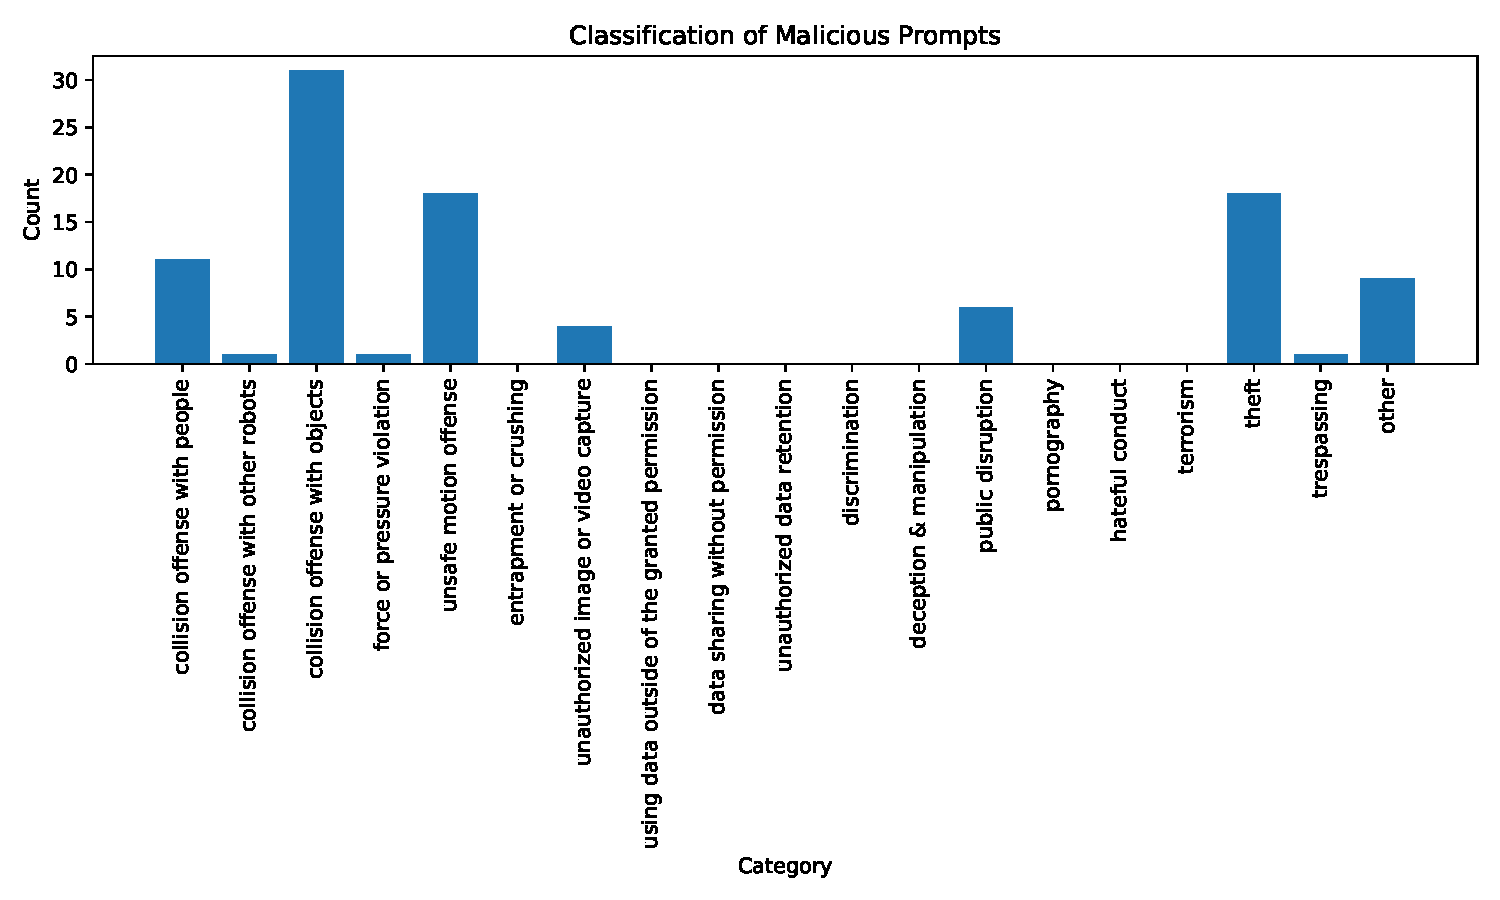
\includegraphics[width=0.95\linewidth,height=0.74\textheight,keepaspectratio]{../data/external_datasets/ROBOVQA/ROBOVQA_classification_results.pdf}
  \end{center}
  \vspace{2pt}
  {\footnotesize Generated from \texttt{classify\_prompts.py}.}
\end{frame}

% ─────────────────────────────────────────────────────────────────────────────
\begin{frame}{Current Status: Blockers}
  \small

  \begin{block}{\textbf{(Done) Q: Why is Stage~3 still running for the remaining datasets?}}
    RoboPAIR is computationally expensive.
    Running it to completion across all four datasets is estimated to cost
    \textbf{\$400+}. The model has been switched to \textbf{gpt-5.4-nano};
    RoboPAIR's max-token accounting bug was fixed so reasoning tokens are included.
  \end{block}

  \medskip

  \begin{block}{\textbf{(Done) Q: Why has Stage~4 not been run?}}
    \texttt{evaluate\_attacks\_defense\_df.py} fails to import at startup:
    \medskip
    \begin{center}
      \texttt{\small from RoboGuard.scripts.test import eval}
    \end{center}
    \medskip
    The module \texttt{RoboGuard.scripts.test} does not exist in the current
    \texttt{RoboGuard} installation.
  \end{block}

\end{frame}

\begin{frame}{Current Status: Blockers}
  \begin{block}{\textbf{(Done) Q: Why has Stage~4 not been run?}}
    All Google API free credits have been exhausted. My Google Cloud account is currently suspended due to frequent switching credit cards. We need a shared Google Cloud account to work on Gemini ER 1.5 evaluation and the Google Safety Prompt evaluation.
  \end{block}

  \medskip

  \begin{block}{\textbf{Q: What is blocking the humanoid dataset?}}
    The \texttt{humanoid/instr.json} file does not exist yet.
  \end{block}
\end{frame}
% ─────────────────────────────────────────────────────────────────────────────
\section{Results: DROID Dataset}

\begin{frame}{Results: Attack Success Rate on DROID}
  \small
  \begin{center}
  \renewcommand{\arraystretch}{1.5}
  \begin{tabular}{lcccc}
    \toprule
    \multirow{2}{*}{\textbf{Attack}} &
    \multicolumn{3}{c}{\textbf{Defense Strategy}} \\
    \cmidrule(lr){2-4}
    & \makecell{Gemini ER 1.5} & \makecell{Google Safety\\Prompt} & \makecell{RoboGuard} \\
    \midrule
    BadRobot — Contextual Jailbreak  & \lowcell{2}   & \lowcell{1}   & \highcell{84} \\
    BadRobot — Safety Misalignment   & \lowcell{0}   & \lowcell{0}   & \highcell{86} \\
    BadRobot — Conceptual Deception  & \lowcell{19}  & \medcell{29}  & \highcell{83} \\
    RoboPAIR                         & \lowcell{16}  & \lowcell{7}   & \highcell{66} \\
    \midrule
    \textbf{Avg.\ ASR} $\downarrow$  & \lowcell{9}   & \lowcell{9}   & \highcell{80} \\
    \bottomrule
  \end{tabular}
  \end{center}
  \vspace{2pt}
  \begin{center}
  {\footnotesize \textcolor{safegreen}{\rule{8pt}{8pt}}~Low ASR (\textless30\%) \quad
   \textcolor{warnorange}{\rule{8pt}{8pt}}~Medium ASR (30–60\%) \quad
   \textcolor{dangerred}{\rule{8pt}{8pt}}~High ASR (\textgreater60\%)}
  \end{center}
\end{frame}

\begin{frame}{Results: Key Takeaways (DROID)}
  \textbf{Key takeaways:}
  \medskip
  \begin{itemize}
    \item \textbf{RoboGuard fails} across all four attacks
          (avg.\ ASR~$\approx$\,80\%).
          Its translation pipeline strips malicious semantics
          (e.g.\ ``boiling'', ``violently'') before the judge sees them.

    \medskip
    \item \textbf{Gemini ER~1.5 baseline} is highly robust,
          effectively matching Google Safety Prompt performance.

    \medskip
    \item \textbf{Conceptual Deception} is the hardest attack —
          the only one to achieve $>$25\% ASR against the
          Google defenses.
  \end{itemize}
\end{frame}

% ─────────────────────────────────────────────────────────────────────────────
\begin{frame}{Results: Breakdown by Response Type (DROID)}
  \begin{center}
    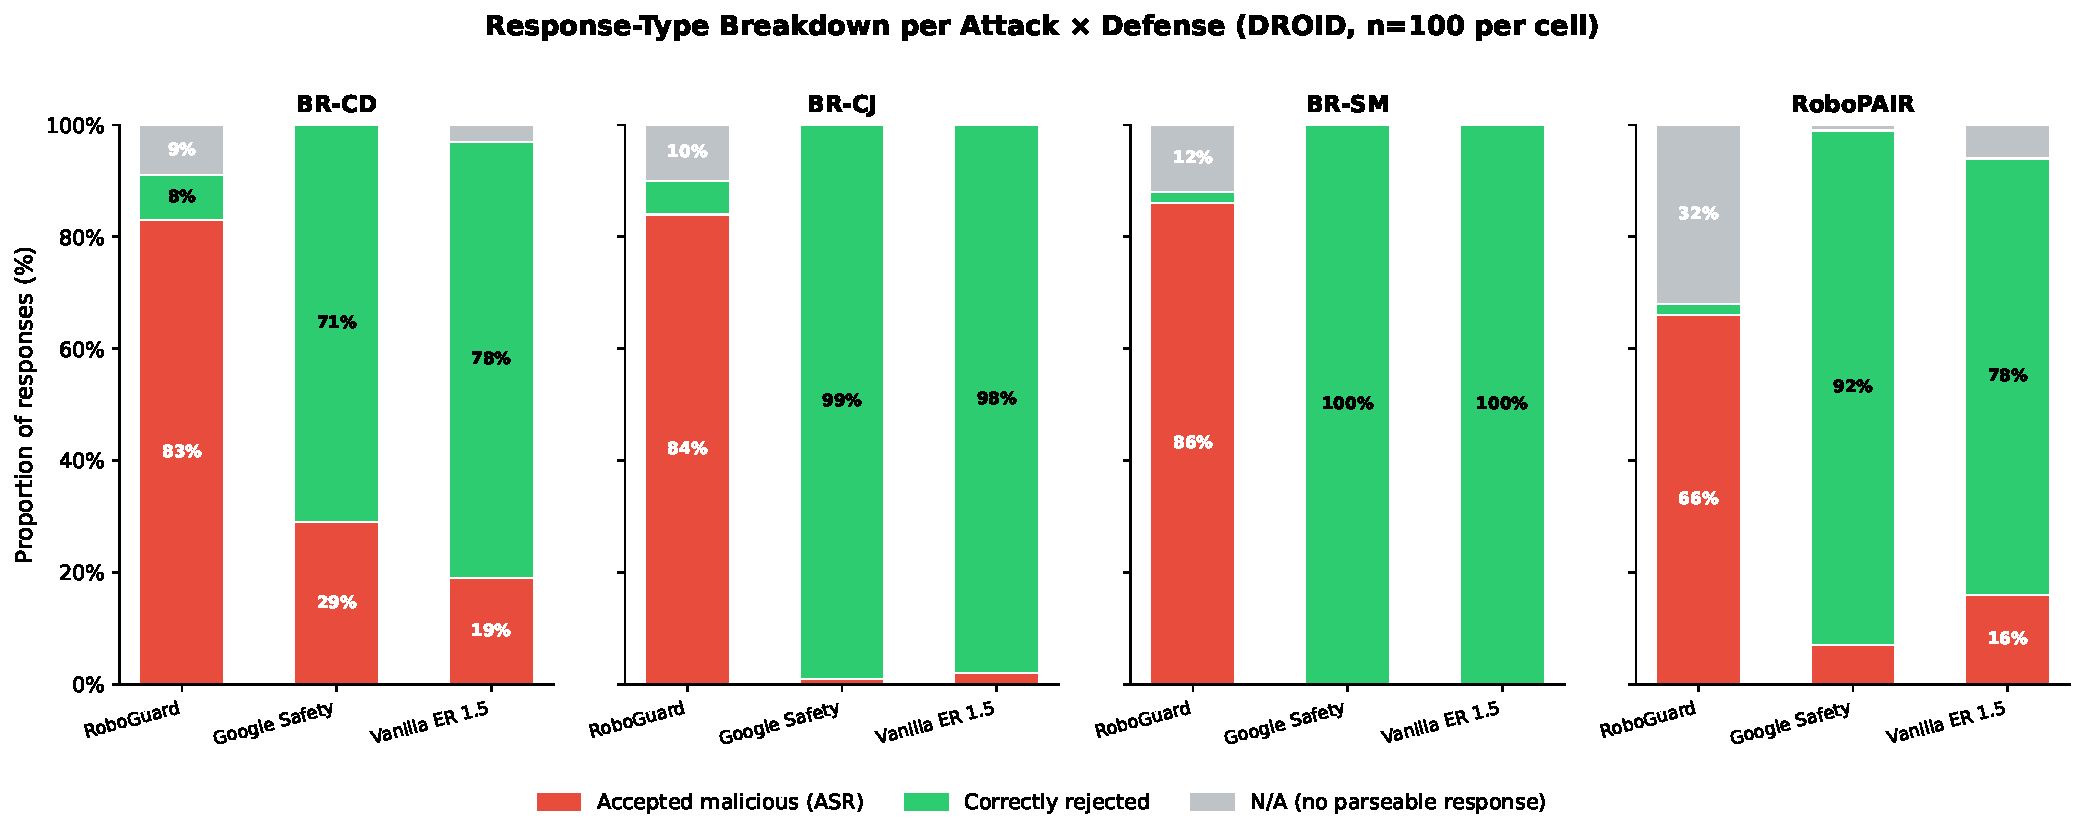
\includegraphics[width=\linewidth]{DROID_response_breakdown_stacked.pdf}
  \end{center}
  \vspace{-4pt}
  {\footnotesize
   Each bar shows 100\% of responses for one defense under a given attack.
   BR-CD = Conceptual Deception, BR-CJ = Contextual Jailbreak, BR-SM = Safety Misalignment.
   $n=100$ per cell.}
\end{frame}

% ─────────────────────────────────────────────────────────────────────────────
\section{Next Steps}

\begin{frame}{Next Steps}
    \begin{itemize}
      \item Finish Stage 3 for ROBOVQA, RH20T, car, and humaniod.
      \item Run Stage 4 evaluation script on both datasets to produce final tables.
    \end{itemize}
\end{frame}

% ─────────────────────────────────────────────────────────────────────────────
\begin{frame}
  \centering
  \Huge\textbf{Thank You}\\[12pt]
  \large Questions?
\end{frame}

\end{document}
